\documentclass{beamer}
\usetheme{Darmstadt}
\usepackage{amssymb}
\usepackage{graphicx}

\newcommand{\nat}{\mathbb{N}}
\newcommand{\ints}{\mathbb{Z}}
\newcommand{\intersection}{\ensuremath{\cap}}
\newcommand{\emptyword}{\ensuremath{\epsilon}}
\newcommand{\len}[1]{\ensuremath{|#1|}}
\newcommand{\union}{\ensuremath{\cup}}

\title{Introduction to Automata Theory}
\author{Sannidhi}
\institute{IISc Bangalore}

\begin{document}



\begin{frame}
\frametitle{Language accepted by a 2-way DFA is regular}
\begin{itemize}
\item Claim: The language accepted by a 2-way finite automaton is regular
\item We will prove this using Myhill-Nerode theorem
\item Recall that the Myhill-Nerode theorem states that a language is regular if and only if the canonical equivalence relation has finitely many equivalence classes
\end{itemize}
\end{frame}

\begin{frame}
\frametitle{Language accepted by a 2-way DFA is regular}
\begin{itemize}
\item Let $M = (Q, \Sigma, \vdash, \dashv, \delta, s, t, r)$ be a 2-way finite automaton
\item Let $w = xz$ be a string in $\Sigma^*$
\item As the automaton is 2-way, its read head can cross the boundary between $x$ and $z$ several times.
\item Consider the function $T_x : (Q\cup\{\bullet\}) \rightarrow (Q\cup\{\bot\})$
\item If the automaton goes to state $q$ when it first crosses the boundary between $x$ and $z$, define $T_x(\bullet) = q$
\item If the read head never crosses the boundary between $x$ and $z$, define $T_x(\bullet) = \bot$
\end{itemize}
\end{frame}

\begin{frame}
\frametitle{Language accepted by a 2-way DFA is regular}
\begin{itemize}
\item Suppose the read head comes back from $z$ to $x$ and reaches state $q$
\item Then it may either go back to $z$ reaching state $p$, in which case define $T_x(q) = p$
\item Else, it may never go back to $z$, in which case define $T_x(q) = \bot$
\item Note that the function $T_x$ is well-defined as the automaton is deterministic
\item Also, $T_x$ depends only on $x$ and is independent of $z$
\item And if $y$ is another string in $\Sigma^*$ such that $T_x = T_y$, then $yz$ is accepted by the automaton if and only if $xz$ is accepted by the automaton
\end{itemize}
\end{frame}

\begin{frame}
\frametitle{Language accepted by a 2-way DFA is regular}
\begin{itemize}
\item Hence, $xRy$ if and only if $T_x = T_y$ becomes a canonical equivalence relation
\item Since the number of unique functions is finite (at most $(k+1)^{k+1}$), the canonical equivalence relation has finitely many equivalence classes
\item Hence the language accepted by the 2-way DFA is regular
\end{itemize}
\end{frame}

\begin{frame}
\frametitle{Example}
\begin{itemize}
\item Let us consider an example of a 2-way DFA accepting the language $L = \{x\in\{a,b\}^* | \#a(x) \text{ is a multiple of 3 and } \#b(x) \text{ is even}\}$
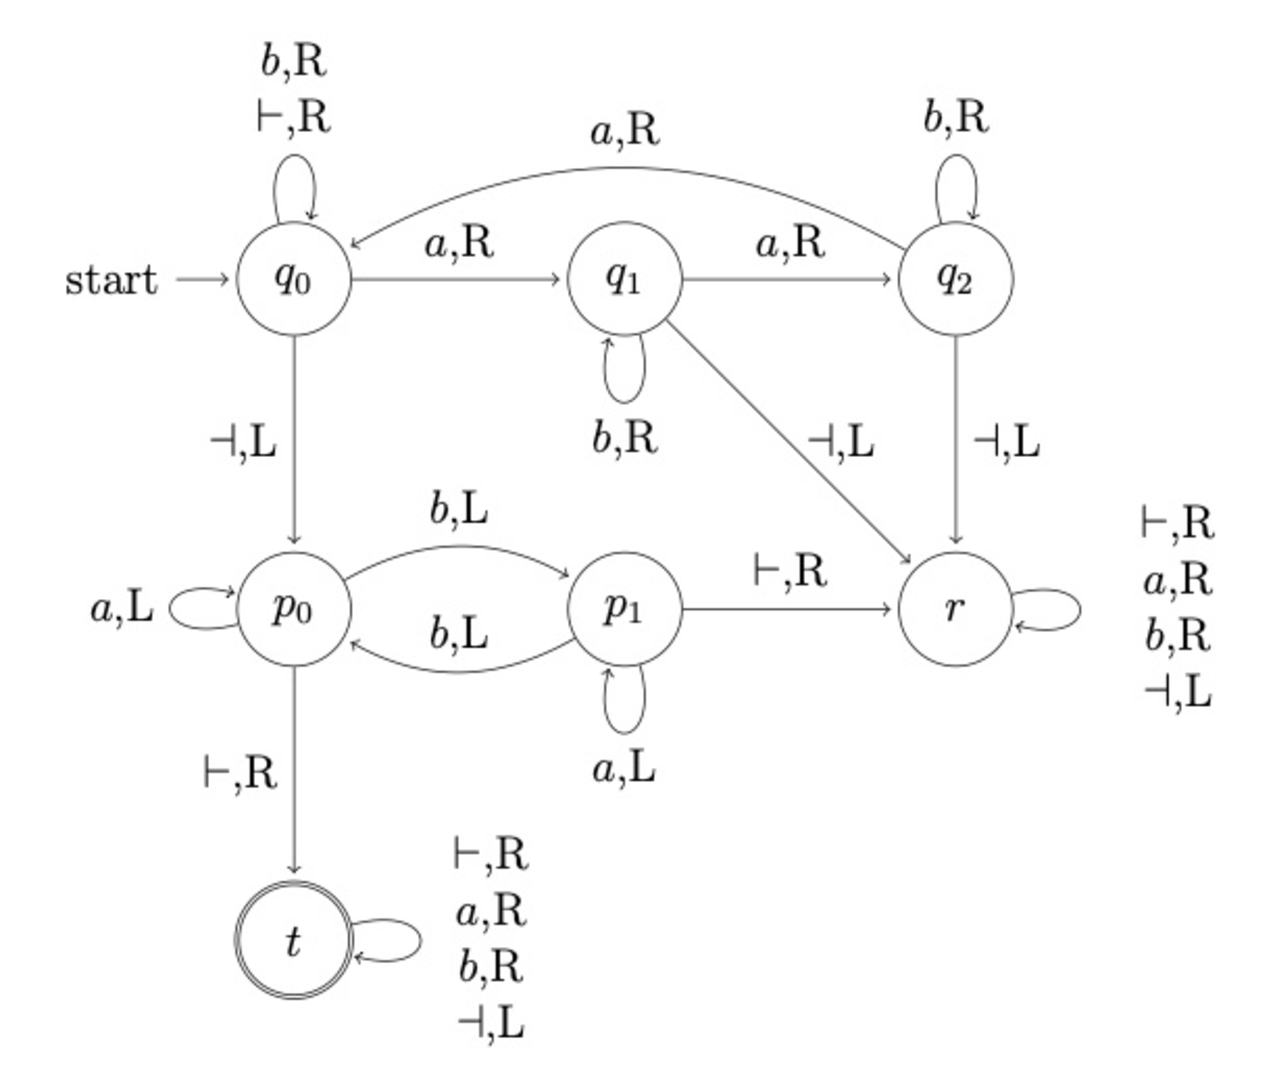
\includegraphics[width=0.6\textwidth]{dfa4.pdf}
\end{itemize}
\end{frame}

\begin{frame}
\frametitle{Example}
\begin{itemize}
\item For any $x\in\{a,b\}^*$,
\item If $\#a(x) = k \mod 3$, then $T_x(\bullet) = p_k$
\item If $\#b(x) = 0 \mod 2$, then $T_x(p_0) = t$ and $T_x(p_1) = r$
\item If $\#b(x) = 1 \mod 2$, then $T_x(p_0) = r$ and $T_x(p_1) = t$
\item And $T_x(t) = t$, $T_x(r) = r$
\item Hence, the canonical equivalence relation has 6 equivalence classes and the language is regular
\end{itemize}
\end{frame}

\begin{frame}
\frametitle{Constructing DFA from 2-way DFA}
\begin{itemize}
\item Once we have the canonical equivalence relation, we can easily construct a DFA.
\item Let $M = (Q, \Sigma, \vdash, \dashv, \delta, s, t, r)$ be a 2-way finite automaton
\item Let $Q'$ be the set of all equivalence classes of the canonical equivalence relation
\item $s' = T_{\emptyword}$
\item $\delta'(T_x, a) = T_xa$
\item $F' = \{T_x|x\in L(M)\}$
\item DFA $M' = (Q', \delta', s', F')$ will accept the same language as the 2-way DFA $M$
\end{itemize}
\end{frame}

\begin{frame}
\frametitle{Example}
\begin{itemize}
\item The DFA accepting the same language as the 2-way DFA is as follows:
\end{itemize}
\begin{figure}
    \centering
        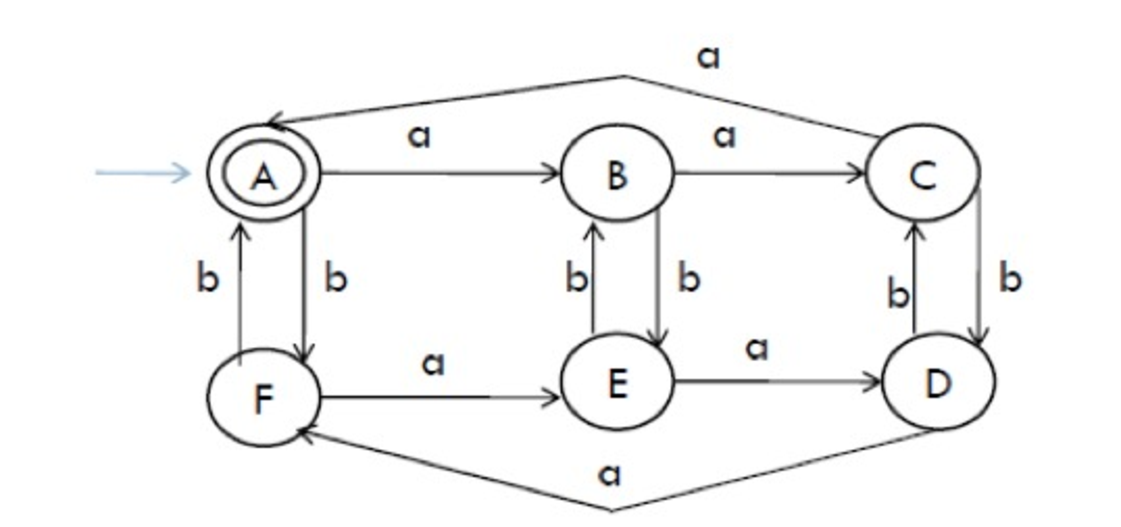
\includegraphics[width=0.6\textwidth]{dfa5.pdf}
\end{figure} 
\end{frame}

\end{document}
